\documentclass[a4paper,10pt]{report}
\usepackage[francais]{babel}
\usepackage{ucs}
\usepackage[utf8x]{inputenc}
\usepackage[T1]{fontenc}
\usepackage[pdftex]{graphicx}
\usepackage{xcolor}
\usepackage{textcomp}
\usepackage[top=2cm, bottom=2cm, left=1.5cm, right=1.5cm]{geometry}
\usepackage{amsmath} 
\usepackage{amssymb}
\usepackage{mathrsfs}
\usepackage{graphicx}
\usepackage{pgfgantt}

\usepackage{listings}
\definecolor{colKeys}{rgb}{0,0,1}
\definecolor{colIdentifier}{rgb}{0,0,0}
\definecolor{-}{rgb}{0,0.5,1}
\definecolor{colString}{rgb}{0.6,0.1,0.1}
\definecolor{colBack}{rgb}{0.9,0.9,0.9}
\definecolor{colComments}{rgb}{0.5,0.5,0.5}
\definecolor{mygreen}{RGB}{28,172,0} % color values Red, Green, Blue
\definecolor{mylilas}{RGB}{170,55,241}


\lstdefinestyle{customc}
{
  belowcaptionskip=1\baselineskip,
  breaklines=true,
  frame=L,
  xleftmargin=\parindent,
  language=C,
  numbers=left,
  showstringspaces=false,
  basicstyle=\footnotesize\ttfamily,
  keywordstyle=\bfseries\color{green!40!black},
  commentstyle=\itshape\color{purple!40!black},
  identifierstyle=\color{blue},
  stringstyle=\color{orange},
  tabsize=4,
}

\lstdefinestyle{customasm}
{
  belowcaptionskip=1\baselineskip,
  frame=L,
  xleftmargin=\parindent,
  language=[x86masm]Assembler,
  basicstyle=\footnotesize\ttfamily,
  commentstyle=\itshape\color{purple!40!black},
}

\lstset{language=Matlab,%
    %basicstyle=\color{red},
    breaklines=true,%
    morekeywords={matlab2tikz},
    keywordstyle=\color{blue},%
    morekeywords=[2]{1}, keywordstyle=[2]{\color{black}},
    identifierstyle=\color{black},%
    stringstyle=\color{mylilas},
    commentstyle=\color{mygreen},%
    showstringspaces=false,%without this there will be a symbol in the places where there is a space
    numbers=left,%
    numberstyle={\tiny \color{black}},% size of the numbers
    numbersep=9pt, % this defines how far the numbers are from the text
    emph=[1]{for,end,break},emphstyle=[1]\color{red}, %some words to emphasise
    %emph=[2]{word1,word2}, emphstyle=[2]{style},    
}

\newcommand{\R}{\mathbb{R}}
\newcommand{\N}{\mathbb{N}}

\lstset{escapechar=@,style=customc}

% Title Page
\title{Rapport MT44\\\huge{TP3}}
\author{Nicolas Fleurot\\Tony Duong}

\begin{document}
\maketitle

\tableofcontents

\chapter*{Introduction}
\addcontentsline{toc}{chapter}{Introduction}

Dans ce TP, on s’intéresse au calcul numérique d’intégrales. Deux approches de la problématique de l’intégration sont proposées, les méthodes d’intégration dîtes classiques et les méthodes gaussiennes. Bien que profondément différentes dans leur construction, ces deux approches s’appuient sur les acquis de l’interpolation vue au TP1. Ce TP commence donc par la mise en oeuvre des méthodes d’intégration classiques et se finira sur les méthodes d’intégration gaussienne.


\chapter*{Partie 1 : Mise en oeuvre des méthodes d'intégration classiques}
\addcontentsline{toc}{chapter}{Partie 1 : Mise en oeuvre des méthodes d'intégration classiques}

\section*{Introduction}
\addcontentsline{toc}{section}{Introduction}

Soient $A$ et $B$ deux réels tels que $A < B$, $f$ une fonction de $[A;B]$ dans $\R$. On désire obtenir une approximation de l'intégrale de $f$ sur $[A;B]$ par les méthodes  classiques d'intégration (méthodes des rectangles, des milieux, des trapèzes et de   Simpson) en prenant $N$ sous-intervalles ($N$ entier naturel non nul). On considère le    pas de discrétisation défini par $h = \frac{(B - A)}{N}$.

\section*{Question a}
\addcontentsline{toc}{section}{Question a}

\subsection*{Rappel}
\addcontentsline{toc}{subsection}{Rappel}

Écrire la fonction Matlab \textit{integ\_classique(type, A, B, N, f )} qui renvoie la valeur $I$ de l’intégrale (supposée existée) à partir du type d’intégration choisi parmi les méthodes classiques, de la fonction $f$ , de l’intervalle d’intégration $[A, B]$ et du nombre $N$ de points. La fonction $f$ , passée en paramètre, désignera une chaîne; elle représente alors une fonction "mathématique" ordinaire.

\subsection*{Théorie}
\addcontentsline{toc}{subsection}{Théorie}

Soit $f$ une fonction régulière sur $[A, B]$ (on supposera $f$ de classe $C^{4}$) et $n$ et $N$ deux entiers naturels.

\begin{itemize}
\item On découpe $[A, B]$ en sous-intervalles à pas constant $h$ ($h$ appartient à $\R^{+*}$), notés $[x_i, x_{i+1}]$, avec $x_0 = A$ et $x_N = V$ et pour tout $i$ appartient à ${0,...,N-1}$, $x_{i+1}-x_i = h$
\item Sur chaque sous-intervalle $[x_i, x_{i+1}]$, on considère la fonction $p_{i,n}$ qui interpole $f$ en des points ${x_{i,0} ,..., x_{i,n}}$ en nombre suffisant. A cette fonction, on applique les résultats de l’intégration sur un intervalle élémentaire.

\item On obtient alors, la valeur approchée de intégrale de $A$ vers $B$ de $f(x) dx$  est somme de $N$ valeurs approchées élémentaires

\begin{eqnarray}
\int_{A}^{B} f(x) \, \mathrm{d}x &\simeq& I^{N}_{R} = h \sum_{\substack{i=0}}^{N-1} f \left(x_i\right)\\
\int_{A}^{B} f(x) \, \mathrm{d}x &\simeq& I^{N}_{M} = h \sum_{\substack{i=0}}^{N-1} f \left(x_i + \frac{h}{2}\right)\\
\int_{A}^{B} f(x) \, \mathrm{d}x &\simeq& I^{N}_{T} = \frac{h}{2}(f(A)+f(B))+h \sum_{\substack{i=1}}^{N-1} f \left(x_i\right)\\
\int_{A}^{B} f(x) \, \mathrm{d}x &\simeq& I^{N}_{S} = \frac{h}{6}\left[f(A)+f(B)+2\sum_{\substack{i=1}}^{N-1}f(x_i) + 4\sum_{\substack{i=0}}^{N-1}f\left(x_i + \frac{h}{2}\right)\right]
\end{eqnarray}

\end{itemize}
\newpage
\subsection*{Source}
\addcontentsline{toc}{subsection}{Source}

\begin{center}
	\lstinputlisting[caption=integ\_classique, language=Matlab]{integ_classique.m}
	\lstinputlisting[caption=integ\_rectangle, language=Matlab]{integ_rectangle.m}
	\lstinputlisting[caption=integ\_milieux, language=Matlab]{integ_millieu.m}
	\lstinputlisting[caption=integ\_trapeze, language=Matlab]{integ_trapeze.m}
	\lstinputlisting[caption=integ\_simpson, language=Matlab]{integ_simpson.m}
\end{center}

\subsection*{Test}
\addcontentsline{toc}{subsection}{Test}


\section*{Question b}
\addcontentsline{toc}{section}{Question b}

\subsection*{Rappel}
\addcontentsline{toc}{subsection}{Rappel}

Pour le calcul d’intégrales connues, par exemple :

\begin{eqnarray}
I_1 &=& \int_{0}^{\frac{\pi}{2}}\sin(x)dx\\
I_2 &=& \int_{0}^{1}\frac{1}{1 + x^2}dx\\
I_3 &=& \int_{0}^{1}x^3 + xdx
\end{eqnarray}

lancer l’exécution de \textit{integ\_classique()} pour différentes valeurs de $N$.
Comparer les valeurs approchées obtenues à leur valeur exacte. Quelle méthode vous parait la plus performante ? Quel critère objectif vous permet-il de justifier cela ? Que remarquez-vous de particulier pour l’intégrale $I_3$ ? Les résultats obtenus sont-ils conformes aux calculs d’erreur de chacune des méthodes, établis en TD.
Produire une (ou des) représentation(s) graphique(s) qui permette(nt) de visualiser les performances comparées des différentes méthodes.

\subsection*{Théorie}
\addcontentsline{toc}{subsection}{Théorie}

L’erreur méthodique globale pour chacune des méthodes est obtenue en sommant les N valeurs d’erreurs élémentaires. 

On obtient alors,

\begin{eqnarray}
E^{N}_{R} &=& h \frac{B-A}{2}f^{(1)}(\eta) \text{ avec } \eta \in ]A, B[\\
E^{N}_{M} &=& h^2 \frac{B-A}{24}f^{(2)}(\eta) \text{ avec } \eta \in ]A, B[\\
E^{N}_{T} &=& -h^2 \frac{B-A}{12}f^{(2)}(\eta) \text{ avec } \eta \in ]A, B[\\
E^{N}_{R} &=& -\left(\frac{h}{4}\right)^4 \frac{B-A}{180}f^{(4)}(\eta) \text{ avec } \eta \in ]A, B[
\end{eqnarray}

\newpage
\subsection*{Test}
\addcontentsline{toc}{subsection}{Test}


\begin{figure}[h]
	\begin{center}
		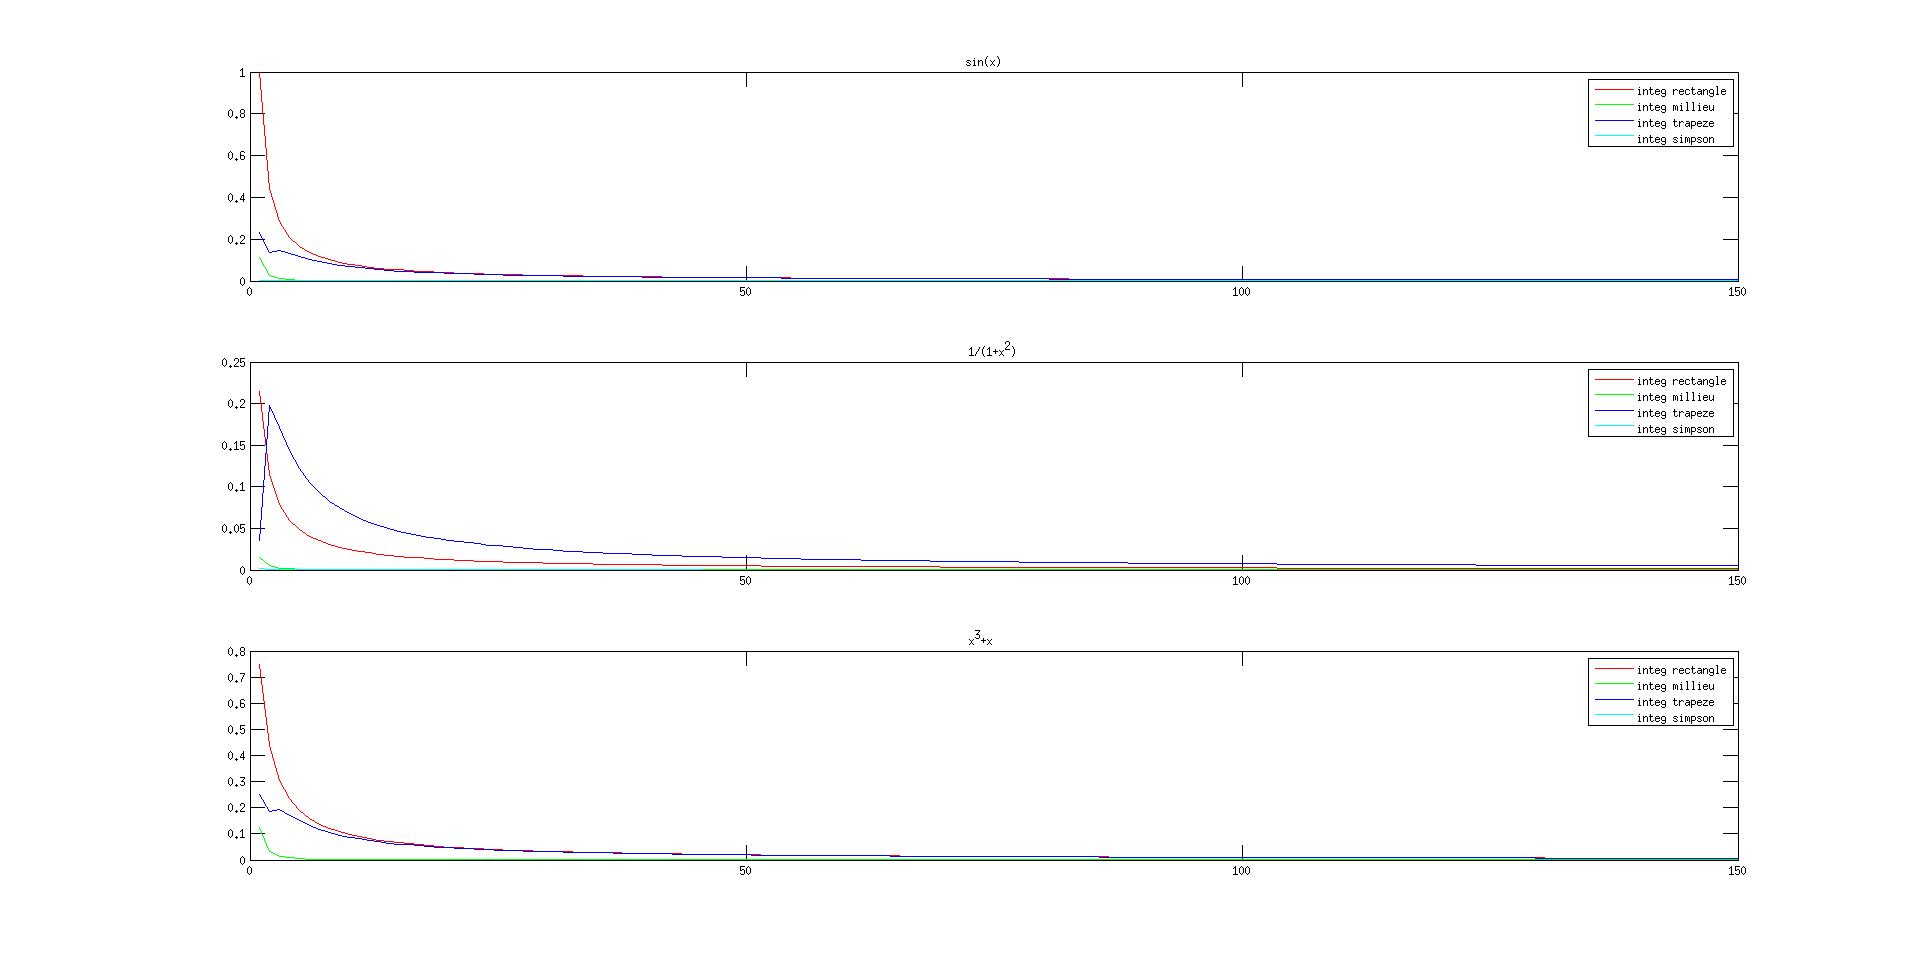
\includegraphics[scale=0.3]{error}
		\caption{Valeur absolue de l'erreur d'intégration}
	\end{center}
\end{figure}

\begin{figure}[h]
	\begin{center}
		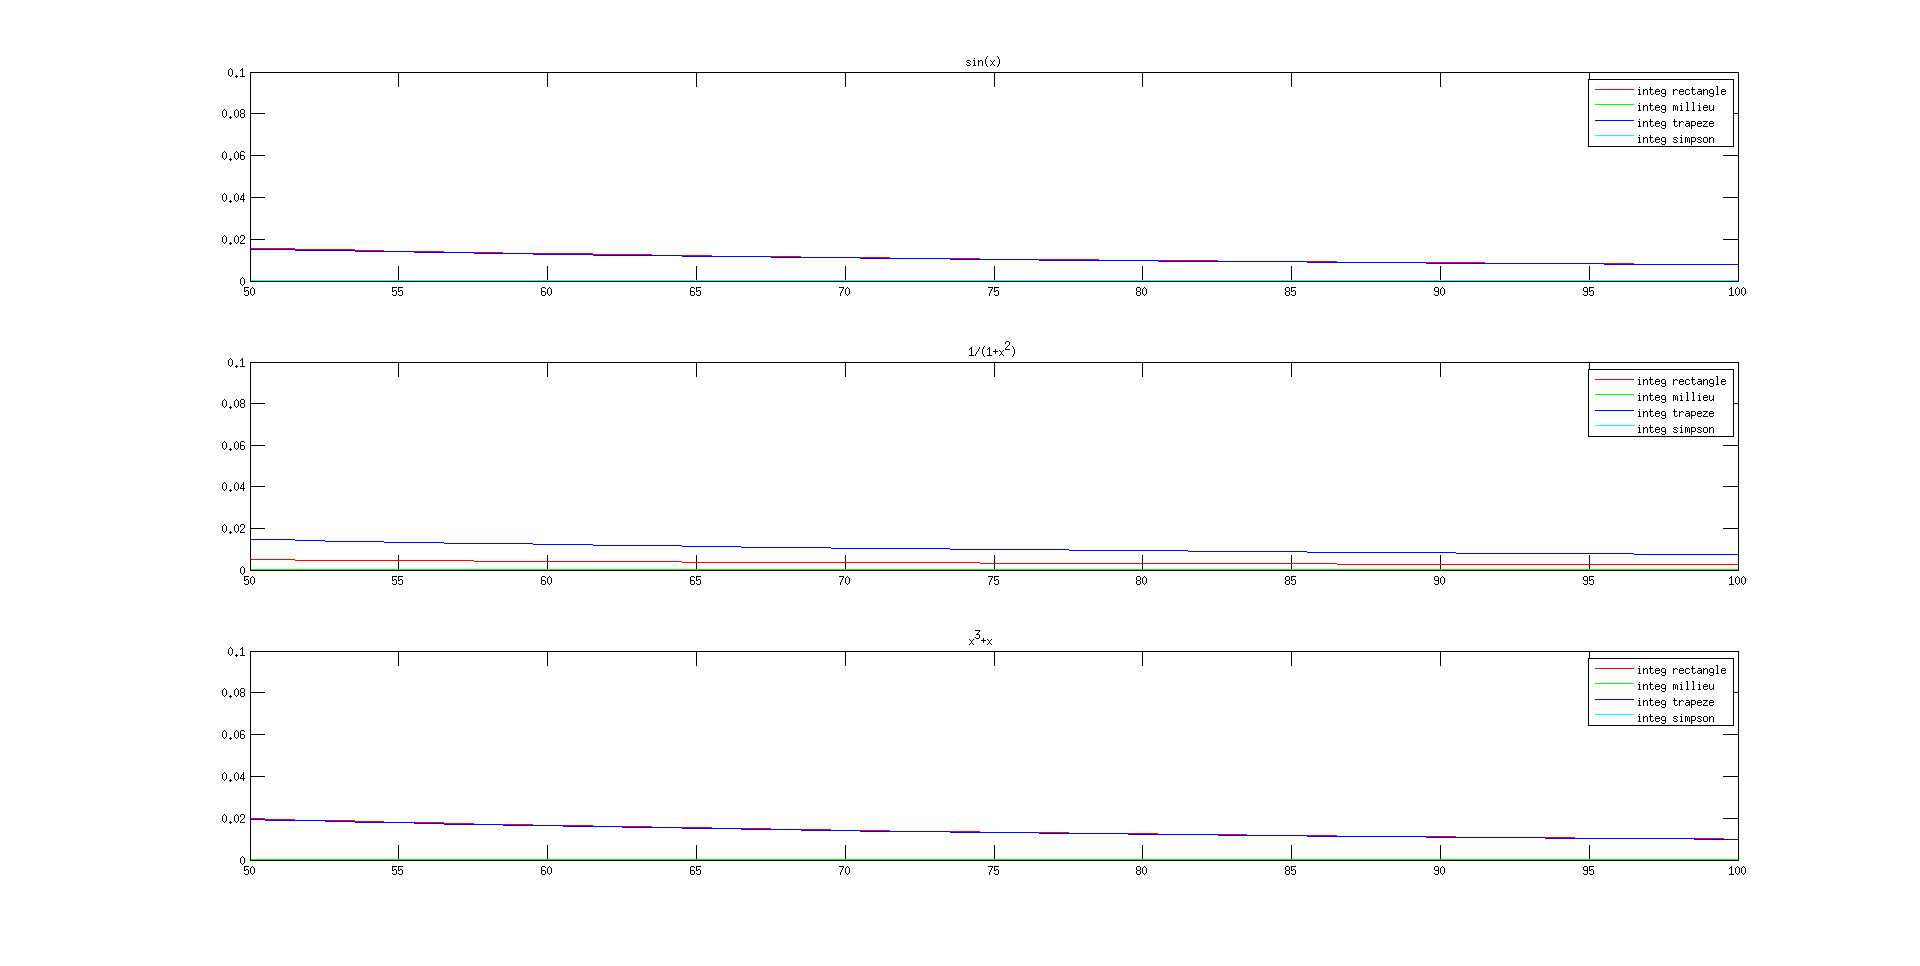
\includegraphics[scale=0.3]{error2}
		\caption{Zoom sur l'erreur d'intégration entre 50 et 100 points}
	\end{center}
\end{figure}

\newpage
\subsection*{Source}
\addcontentsline{toc}{subsection}{Source}

\begin{center}
	\lstinputlisting[caption=integ\_classique, language=Matlab]{test_error.m}
\end{center}

\chapter*{Partie 2 : Intégration gaussienne}
\addcontentsline{toc}{chapter}{Partie 2 : Intégration gaussienne}


\section*{Introduction}
\addcontentsline{toc}{section}{Introduction}

L'objet de cette partie est de préparer, sans qu'il soit nécessairement complet, un “kit d'intégration gaussienne”. On se préoccupera de le rendre opérationnel pour les méthodes de Legendre et Tchebyschev ; les autres cas constitueront le “default” d'un switch a développer ultérieurement.
La structure globale de la fonction d'intégration gaussienne doit exister ; l'utilisateur peut choisir  la méthode a mettre en oeuvre.
On ne réfléchira, qu'une fois le reste du TP terminé, a la reconnaissance de la forme d'intégration gaussienne à utiliser en process automatique !

\section*{Question a}
\addcontentsline{toc}{section}{Question a}

\subsection*{Rappel}
\addcontentsline{toc}{subsection}{Rappel}

Détermination des polynômes orthogonaux Construire la suite des n max (par exemple n max = 20) premiers polynômes orthogonaux de Legendre et Tchebyschev. On utilisera la relation de récurrence fournie en cours ; on rappelle que :

\begin{eqnarray*}
L_0 (x) = 1 \text{, }L_1 (x) = x \text{, } &&\forall k \in \N^* L_{k+1} = \frac{2k+1}{k+1}xL_k (x) - \frac{k}{k+1}L_{k-1}(x)\\
T_0 (x) = 1 \text{, }T_1 (x) = x \text{, } &&\forall k \in \N^* T_{k+1} = 2xT_k (x) - T_{k-1}(x)
\end{eqnarray*}

On stockera les résultats dans des matrices.

\subsection*{Théorie}
\addcontentsline{toc}{subsection}{Théorie}

En mathématiques, une suite de polynômes orthogonaux est une suite infinie de polynômes $p_0(x), p_1(x), p_2(x)$ ... à coefficients réels, dans laquelle chaque $p_n(x)$ est de degré $n$, et telle que les polynômes de la suite sont orthogonaux deux à deux pour un produit scalaire de fonctions donné.

\subsection*{Source}
\addcontentsline{toc}{subsection}{Source}

\begin{center}
	\lstinputlisting[caption=Polynome de Legendre, language=Matlab]{polynome_legendre.m}
	\lstinputlisting[caption=Polynome de Tchebyschev, language=Matlab]{polynome_tchebyschev.m}
\end{center}

\section*{Question b}
\addcontentsline{toc}{section}{Question b}

\subsection*{Rappel}
\addcontentsline{toc}{subsection}{Rappel}

Pour les différentes familles de polynômes orthogonaux prises en compte au paragraphe précédent déterminer leurs zéros et les stocker dans une matrice appropriée.

\subsection*{Théorie}
\addcontentsline{toc}{subsection}{Théorie}

Les zéros des polynômes orthogonaux nous seront indispensables pour calculer l’intégrale numérique.

\subsection*{Source}
\addcontentsline{toc}{subsection}{Source}

\begin{lstlisting}[language=Matlab]
roots(sym2poly((poly_legendre(i)))) % Racines des polynomes de Legendre
roots(sym2poly((poly_tchebyschev(i)))) % Racines des polynomes de  Tchebyschev
\end{lstlisting}

\section*{Question c}
\addcontentsline{toc}{section}{Question c}

\subsection*{Rappel}
\addcontentsline{toc}{subsection}{Rappel}

Détermination des coefficients d’intégration.\\
On rappelle qu'en intégration gaussienne

\begin{equation*}
\int_{a}^{b}f(x)dx = \int_{a}^{b}r(x) w(x)dx \simeq \sum_{\substack{i=0}}^{n}D_i r(x_i)
\end{equation*}

où $[a, b]$ désigne l’intervalle conventionnel d’intégration pour la méthode étudiée, $r$ la régularisée de la fonction à intégrer, $w$ la fonction poids associée, $D_i$ les coefficients cherchés et $x_i$ les zéros déterminés à la question précédente.
À partir des résultats fournis dans le polycopié, déterminer pour chaque méthode prise en compte, les coefficients nécessaires et les stocker.

\subsection*{Théorie}
\addcontentsline{toc}{subsection}{Théorie}

Les zéros des polynômes orthogonaux nous seront indispensables pour calculer l’intégrale numérique. Pour l’intégration de Legendre, ces zéros ne sont pas connus explicitement mais calculés par une méthode numérique. En revanche, pour l’intégration de Tchebyschev, les zéros sont connus explicitement et données par :
    
\begin{equation*}
\forall{i} \in \{0, ..., n\}, x_i = \cos \left(\frac{2i + i}{n + 1}\frac{\pi}{2}\right)
\end{equation*}

\subsection*{Source}
\addcontentsline{toc}{subsection}{Source}

\begin{lstlisting}[caption=Zeros de Legendre, language=Matlab]
zeros_legendre = zeros(nb_points-1, nb_points-1);
for i=2:nb_points
    rootsPoly = double(roots(sym2poly((poly_legendre(i)))));
    zeros_legendre(:, i-1) = [rootsPoly; zeros(nb_points-i, 1)];
end
\end{lstlisting}

\begin{lstlisting}[caption=Zeros de Tchebyschev, language=Matlab]
zeros_tchebyschev = zeros(nb_points-1, nb_points-1);
poly_tchebyschev = polynome_tchebyschev(nb_points);
for i=2:nb_points
    zeros_tchebyschev(:, i-1) = [roots(sym2poly(poly_tchebyschev(i))); zeros(nb_points-i, 1)];
end
\end{lstlisting}

\section*{Question d}
\addcontentsline{toc}{section}{Question d}

\subsection*{Rappel}
\addcontentsline{toc}{subsection}{Rappel}

Intégrer les éléments antérieurs pour calculer une valeur approchée d’intégrales convenables par méthode gaussienne. On écrira une fonction \textit{intégration\_gaussienne(type, nb points, r)} qui renvoie une valeur approchée \\de $I=\int_{a}^{b}r(x)w(x)dx$, à partir de la donnée du type d’intégration gaussienne requis, du nombre
de points à prendre en compte et de la fonction régularisée associée $r$ passée comme une chaîne.
 

\subsection*{Théorie}
\addcontentsline{toc}{subsection}{Théorie}
Pour Gauss-Legendre, 
\begin{equation*}
\forall{i} \in \{0, ..., n\}, W_i = \frac{2}{(n+1)L'_{n+1}(x_i)L_{n}(x_i)}
\end{equation*}

Pour Gauss-Tchebyschev,
\begin{equation*}
\forall{i} \in \{0, ..., n\}, W_i = \frac{\pi}{n+1}
\end{equation*}

\subsection*{Source}
\addcontentsline{toc}{subsection}{Source}


\section*{Question e}
\addcontentsline{toc}{section}{Question e}

\subsection*{Rappel}
\addcontentsline{toc}{subsection}{Rappel}

Pour une ou plusieurs intégrales calculables explicitement, évaluer l’erreur de calcul commise et visualiser cette erreur en fonction du nombre de points considérés.

\subsection*{Théorie}
\addcontentsline{toc}{subsection}{Théorie}

Pour Gauss-Legendre, l’erreur commise est donnée par :

\begin{equation*}
E_{n+1} = r^{(2n+2)}(\xi) \frac{2^{2n+3}\left[(n+1)!\right]^4}{(2n+3)\left[(2n+2)!\right]^3}
\end{equation*}

Pour Gauss-Tchebyschev, l’erreur commise est donnée par :

\begin{equation*}
E_{n+1} = r^{(2n+2)}(\xi) \frac{2\pi}{2^{2n+2}(2n+2)!}
\end{equation*}

\subsection*{Test}
\addcontentsline{toc}{subsection}{Test}

\begin{figure}[h]
	\begin{center}
		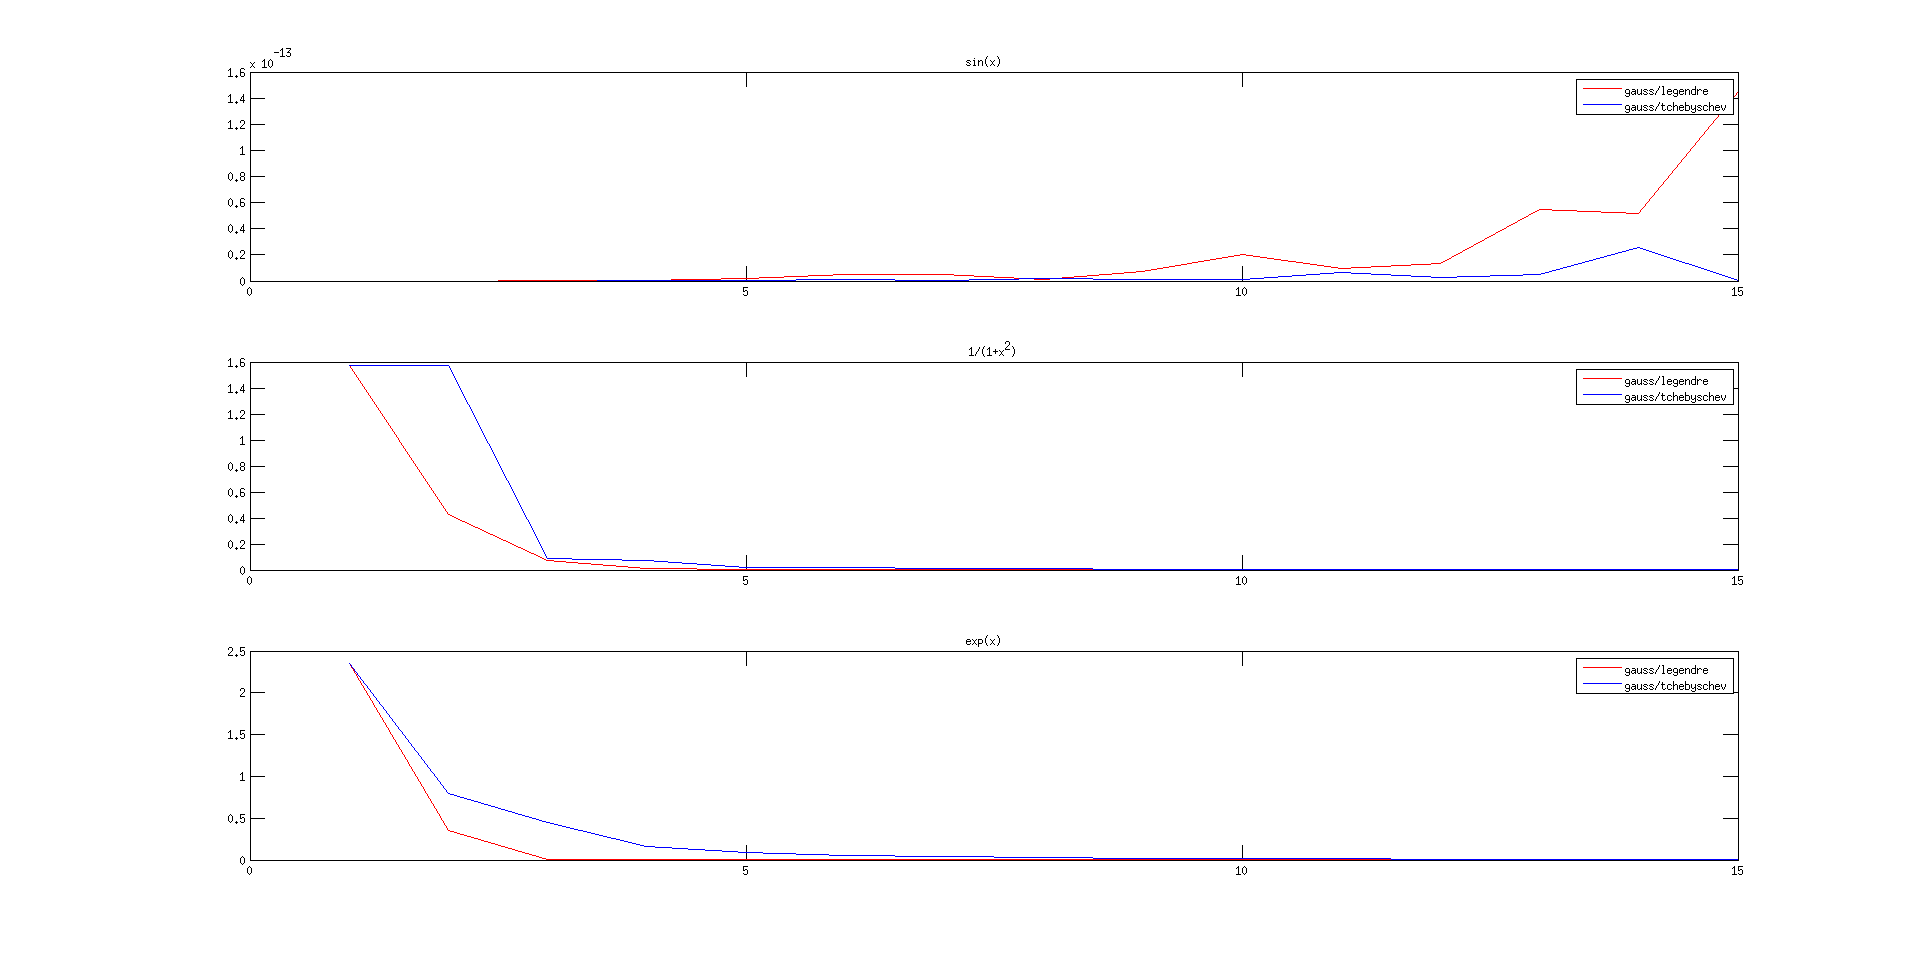
\includegraphics[scale=0.35]{error_gauss}
		\caption{Valeur absolue de l'erreur d'intégration}
	\end{center}
\end{figure}

\subsection*{Source}
\addcontentsline{toc}{subsection}{Source}

\begin{center}
	\lstinputlisting[caption=erreur d'integration de Gauss, language=Matlab]{test_error_gauss.m}
\end{center}

\chapter*{Conclusion}
\addcontentsline{toc}{chapter}{Conclusion}


\end{document}